% Nastavení dokumentu

\documentclass[FM,DP]{tulthesis}  % Diplomová práce fakulty mechatroniky
\usepackage[czech]{babel}  % Česká šablona dokumentu
\usepackage[utf8]{inputenc}  % Česká diakritika
\usepackage{graphicx}  % Tvorba tabulek
\usepackage{float}  % Ukotvení věcí na svém místě (obrázky, tabulky, grafy, ...)
\usepackage{hyperref}  % Klikací odkazy v obsahu a referencích
\usepackage{gensymb}  % Pro stupne celsia
\usepackage{url}  % Pro lomeni adres url

% Titulní stránka

\TULtitle{Inteligentní domovní systém}{Smart home system}
\TULprogramme{N2610}{Elektrotechnika a informatika}{Electrical Engineering and Informatics}
\TULbranch{1802T007}{Informační technologie}{Information Technology}
\TULauthor{Bc. Tomáš Moravec}
\TULsupervisor{doc. Ing. Josef Chaloupka, Ph.D.}
\TULyear{2018}

% Prohlášení

\begin{document}
\ThesisStart{male}

% Poděkování

\begin{acknowledgement}
Děkuji vedoucímu práce panu doc. Ing. Josefu Chaloupkovy, Ph.D. za odborné vedení a poskytnuté informace při zpracování závěrečné diplomové práce.
\end{acknowledgement}

% Abstrakt

\begin{abstractCZ}
Práce se zabývá vytvořením inteligentního domovního systému, určenému ke zpracování dat z bezpečnostních a meteorologických čidel, a řízení vybraných domovních zařízení. Komplexní řešení zahrnuje jak samotný domovní systém, tak mobilní, webovou a desktopovou aplikaci. V úvodu jsou definovány základní pojmy a požadované vlastnosti. Následuje rešerše a výběr vhodných hardwarových a softwarových řešení. Ná základě rešerše je navržen koncept komplexního domovního systému, který je následně realizován v jednotlivých etapách. Výstupem práce je funkční cílové zařízení, které aplikuje zvolené hardwarové i softwarové řešení.

\end{abstractCZ}

\vspace{2cm}

\begin{abstractEN}
Not implemented yet.
\end{abstractEN}

% Seznam zkratek

\tableofcontents
\clearpage

\begin{abbrList}
\textbf{API} & Application Programming Interface, rozhraní pro přístup k aplikaci\\
\textbf{COM} & Communication port, komunikační rozhraní\\
\textbf{GBS} & Glass break detector, detektor rozbití skla\\
\textbf{GPRS} & General Packet Radio Service, služba pro přenos dat v mobilní síti\\
\textbf{GSM} & Groupe Spécial Mobile, globální systém pro mobilní komunikaci\\
\textbf{GUI} & Graphical User Interface, grafické uživatelské rozhraní\\
\textbf{IDE} & Integrated development environment, integrované vývojové prostředí\\
\textbf{IP} & Internet Protocol, internetový protokol\\
\textbf{LAN} & Local Area Network, místní počítačová síť\\
\textbf{LED} & Light-Emitting Diode, dioda emitující světlo\\
\textbf{PIR} & Passive infrared sensor, pasivní infračervené čidlo\\
\textbf{SMS} & Short message service, služba krátkých textových zpráv\\
\textbf{TUL} & Technical University of Liberec, Technická univerzita v Liberci\\
\textbf{USB} & Universal Serial Bus, univerzální sériová sběrnice\\
\end{abbrList}

% Úvod

\chapter{Úvod}
Not implemented yet.

% Inteligentní domovní systém

\chapter{Inteligentní domovní systém}
Inteligentní domovní systém je kombinací zabezpečovacího systému s prvky chytré domácnosti. Nyní se zaměřím na vysvětlení pojmů zabezpečovací systém a inteligentní dům (chytrá domácnost).

% Zabezpečovací systém

\section{Zabezpečovací systém}
Zabezpečovací systém, někdy také elektronická zabezpečovací signalizace, je zařízení, které vizuálně nebo akusticky vyhlašuje poplach a dává na vědomí, že nastaly nějaké potíže nebo došlo ke splnění sledované podmínky \cite{Security alarm}. Jde tedy o zařízení, které slouží k ochraně osob a majetku. Systém je řízen ústřednou a může se spustit analogovou (např. dveřní, či okenní čidlo) i digitální (detektor pohybu) detekcí. Komunikace mezi detektory a ústřednou může být vedena kabelem, bezdrátově anebo kombinací předešlých způsobů, tj. jeden detektor může být připojen kabelem a druhý bezdrátově \cite{Electronic security system}.

\subsection{Ústředna}
Ústředna je „mozek“ celého systému, který je propojen s ostatními prvky systému kabely nebo bezdrátově. Obstarává komunikaci mezi jednotlivými komponenty systému, má v integrované paměti uložené nejdůležitější nastavení \cite{Electronic security system}. V závislosti na připojených komponentech pak může různě reagovat na splnění sledovaných podmínek. Často bývá vybavena jenom tím nejnutnějším pro vyvolání poplachu, to ať už akustického (siréna), nebo tichého (informování majitele) \cite{Security alarm}.

\subsection{Ovladač}
Ovladač je prvek, který slouží k ovládání a případně též k programování ústředny. Dnešní alarmy je možné ovládat několika způsoby. Jako ovladač se nejčastěji používá klávesnice vybavená tlačítky, případně čtečkou (čipovými kartami a přívěšky) nebo též dálkové ovládání. U některých systémů se dá přes klávesnici provést nastavení celého systému. Klávesnice slouží k zastřežení i odstřežení systému \cite{Electronic security signalisation}. Dalšími způsoby je ovládání přes internet, kdy se většinou používá integrované webové rozhraní, ke kterému se uživatel může připojit po zadání hesla, nebo ovládání přes mobil (SMS příkazy) \cite{Bachelor thesis}.

\subsection{Detektor}
Detektor je prvek systému, který je rozmístěn v hlídaném objektu a má za úkol reagovat aktivací při narušení (otevření, pohyb, rozbití atd.) a to tak, že tuto informaci předá ústředně, která ji následně zpracuje \cite{Electronic security signalisation}. Nejčastěji používané detektorové prvky jsou:

\begin{itemize}
\item Magnetický kontakt (dveřní čidlo)
\item Detektor pohybu (PIR detektor)
\item Detektor tříštění skla (GBS detektor)
\item Detektor plynu
\item Infra závora
\end{itemize}

\subsection{Komunikátor}
Komunikátor je zařízení, které odesílá informaci o narušení objektu, případně o odchylce od normálního provozního stavu zabezpečovacího systému, mimo  hlídaný objekt. \cite{Electronic security signalisation}. Nejčastější typy komunikátorů jsou:

\begin{itemize}
\item GSM komunikátor
\item LAN komunikátor
\item Telefonní komunikátor
\item Komunikátor využívající radiové sítě s vyhrazenou frekvencí
\end{itemize}

% Inteligentní dům

\section{Inteligentní dům}
Inteligentní dům, neboli chytrá domácnost znamená možnost ovládání osvětlení, elektroinstalace, termostatu, domácího alarmu, kamer nebo zámku dveří na dálku skrze chytrý telefon, tablet, ale i počítač nebo televizi. Běžně je vše propojeno centální jednotkou, která většinou poskytuje dálkové ovládání skrze internet.

\subsection{Centrální jednotka}
Srdcem chytré domácnosti je centrální jednotka (neboli řídící jednotka), která komunikuje prostřednictvím konkrétního protokolu. K takové jednotce je možné kdykoliv dokupovat další zařízení, a tvořit tak komplexní chytrou domácnost. Ovládání a řízení celého systému je velmi jednoduché a intuitivní. Inteligentní dům se samozřejmě také stará o zabezpečení domácnosti a poskytuje vám kdykoliv a kdekoliv přehled o jejím aktuálním stavu.

\paragraph{Nejčastější typy připojovaných řízení:}
\begin{itemize}
\item Osvětlení
\item Elektroinstalace
\item Termostaty
\item Zabezpečení
\item Kamery
\item Meteostanice
\end{itemize}

% Požadované vlastnosti

\section{Požadované vlastnosti}
V následující části se zaměřím na požadované vlastnosti všech částí inteligentního domovního systému (ekosystém).

\subsection{Domovní systém}
Z úvodní části je zřejmé, že domovní systém obsahuje jak prvky zabezpečovacího systému, tedy musí obsahovat detektory, komunikátor a ústřednu. Zároveň však obsahuje prvky inteligentního domu, tedy musí být schopna monitorovat a řídit různá zařízení v domácnosti. V rámci domovního systému jsou výše zmíněné prvky řízeny ovladačem. V této práci se jedná o desktopovou, mobilní aplikaci a webovou aplikaci. Komunikace bude probíhat přes internet.

\paragraph{Požadavky na domovní systém:}
\begin{itemize}
\item Poskytnutí API
\item Komunikace přes internet
\item Vzdálené ovládání všech připojených zařízení
\item Vzdálená správa a monitoring všech připojených zařízení
\item Spuštění poplachu při splnění podmínek (kontaktování uživatele)
\item Komunikaci s desktopovou, mobilní a webovou aplikací
\end{itemize}

\subsection{Desktopová aplikace}
Desktopová aplikace musí být schopna využít plného potenciálu ústředny, tedy umožnit kompletní správu a nastavování jednotlivých komponent (spínačů a senzorů). Komunikace s ústřednou bude umožněna pomocí sériové linky (COM port), v případě prototypu bude použito připojení skrze USB.

\paragraph{Požadavky na desktopovou aplikaci:}
\begin{itemize}
\item Komunikace po seriové lince
\item Zobrazení seznamu všech připojench komponent
\item Zobrazení všech informací o zvolené komponentě
\item Změna libovolného nastavení všech komponent
\item Sledování aktuálního stavu všech komponent
\item Přidávání nových komponent
\item Odstraňování stávajících komponent
\item Notifikace v případě změny stavů senzorů
\item Změna stavu spínačů
\item Připojování a odpojování od zvolené ústředny
\end{itemize}

\subsection{Mobilní aplikace}
Mobilní aplikace je učena pouze jako monitorovací zařízení, ze kterého bude možné sledovat stavy jednotlivých senzorů, případně spínat veškeré spínací prvky. Její návrh je tedy značně jednodušší oproti komplexnější desktopové aplikaci. Komunikace bude probíhat přes internet.

\paragraph{Požadavky na mobilní aplikaci:}
\begin{itemize}
\item Komunikace přes internet
\item Zobrazení seznamu všech připojench komponent
\item Zobrazení všech informací o zvolené komponentě
\item Sledování aktuálního stavu všech komponent
\item Notifikace v případě změny stavů senzorů
\item Změna stavu spínačů
\item Připojování a odpojování od zvolené ústředny
\end{itemize}

\subsection{Webová aplikace}
Od webové aplikace se očekává možnost sledování aktuálního denní a zobrazení historických dat. Od aplikace se neočekává možnost editace, ani a jakékoliv řízení. Komunikace bude probíhat přes internet.

\paragraph{Požadavky na webovou aplikaci:}
\begin{itemize}
\item Komunikace přes internet
\item Sledování aktuálního stavu všech komponent
\item Zobrazení historických dat
\end{itemize}

\subsection{Komunikační server}
Komunikační server je nutný pro navázání spojení mezi řídící jednotkou a mobilní a webovou aplikací. Od serveru se očekává udržování a správa všech spojení, stejně tak jako propagace zpráv do jejich cílových destinací. Komunikaci je nutné logovat a bude probíhat přes internet.

\paragraph{Požadavky na komunikační server:}
\begin{itemize}
\item Komunikace přes internet
\item Udržování stálého spojení s klienty
\item Zajištění komunikace mezi klienty
\item Logování probíhající komunikace
\end{itemize}

% Zvolené řešení

\chapter{Zvolené řešení}

\section{Domovní systém}
Jak již bylo řečeno, domovní systém je kombinací zabezpečovacího zařízení a spínacích prvků. Všem těmto částem se budu věnovat níže, kde vyberu nejvhodnější varianty.

\subsection{Řídící jednotka}
Řídící jednotka musí být schopna spravovat všechny připojené detektory, senzory a spínací prvky, a komunikovat s desktopovou a mobilní aplikací. a zároveň musí řídit a zpracovávat jednotlivé komponenty. Již ze zadání diplomové je zřejmé, že řídící jednotkou bude vývojová platforma Arduino \cite{Pruvodce arduinem}, která je se svými periferiemi \cite{Arduino schematic} a čipem Atmega \cite{Atmega datasheet}, případně ARM Cortex-M3, více než vhodnou pro tyto účely. Firmware řídící jednotky bude psán v jazyku  C++ s nadstavbou Wiring (knihovna pro řízení hardwaru) \cite{Wiring} a vývoj bude probíhat v prostředí Visual Studio 2017 s rozšířením Visual Micro \cite{Visual Micro}, které poskytuje zvýrazňování syntaxe knihovny Wiring a umožňuje komplikaci a nahrávání kódu přímo na desku Arduino. Komunikace bude probíhat skrze mobilní datovou síť.

\paragraph{Zvolená řídící jednotka:}
\begin{itemize}
\item Arduino DUE (914 Kč s DPH), (\url{arduino-shop.cz})
\end{itemize}

\begin{figure}[H]
\begin{center}
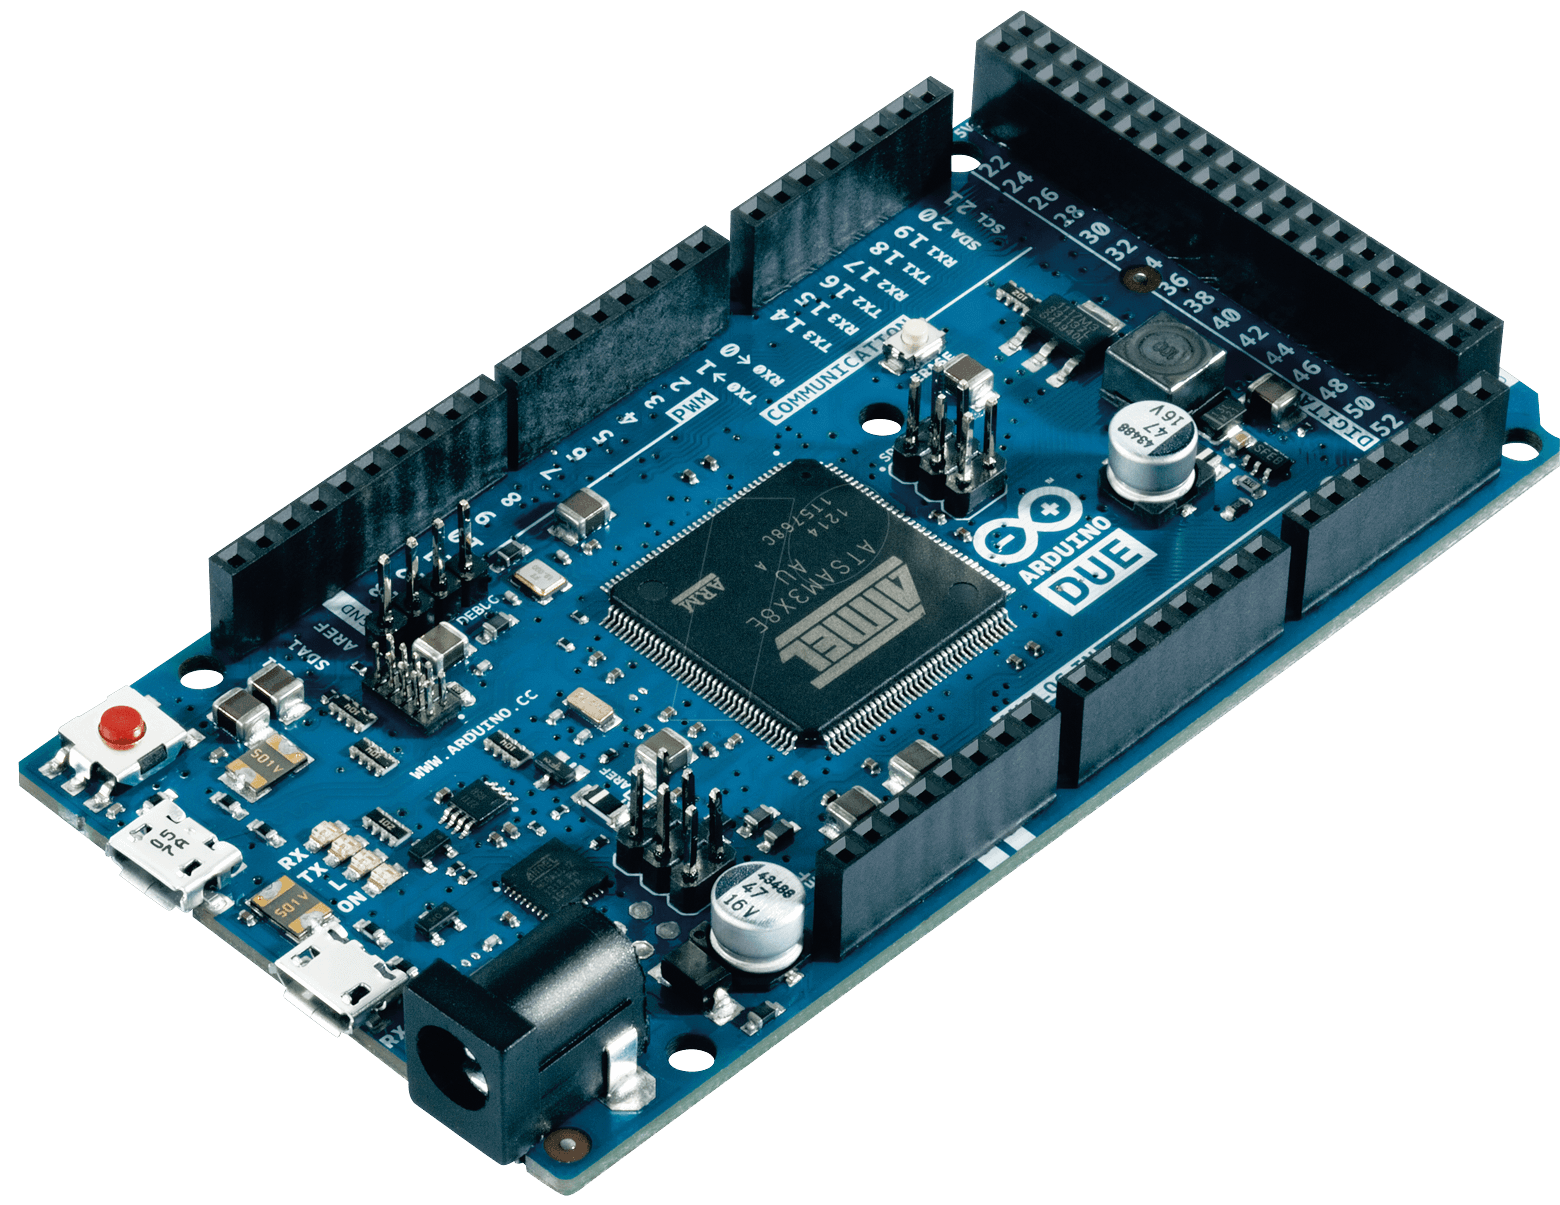
\includegraphics[width=0.5\textwidth]{images/arduinoDue.png}
\caption{Vývojová platforma Arduino DUE}
\label{image}
\end{center}
\end{figure}

\subsection{Detektory}
Detektory jsou všechny velmi podobné a proto stačí připravit implementaci jejich snímání. V případě detektorů musí být možné připojit libovolný detektor, který lze nastavit jako spínací (normálně rozepnutý), nebo rozpínací (normálně sepnutý). Pro testovací účely byly zvoleny dva detektory, každý jednoho typu.

\paragraph{Zvolené detektory:}
\begin{itemize}
\item Dveřní čidlo (rozpínací), (poskytl vedoucí)
\item PIR detektor (spínací), (25 Kč s DPH), (\url{aliexpress.com})
\end{itemize} 

\begin{figure}[H]
\begin{center}
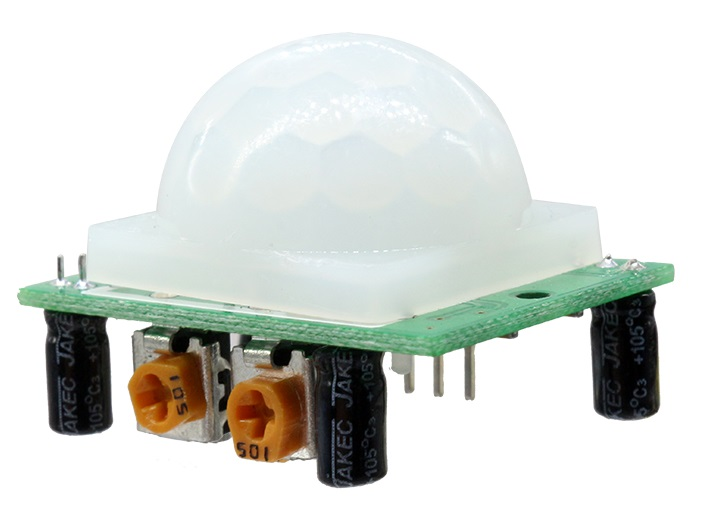
\includegraphics[width=0.3\textwidth]{images/PIR.jpg}
\caption{Detektor pohybu (PIR detektor)}
\label{image}
\end{center}
\end{figure}

\subsection{Spínací prkvy}
U spínacích prvků není nutné volit jednotlivé komponenty, ale stačí připravit implementaci jejich spínání. Poté je možné připojit libovolnou spínatelnou součástku.

\subsection{Komunikátor}
Požadavek na komunikátor je přenos dat na server přes mobilní data. Původní zadání jako komunikátor určuje mobilní telefon, pomocí kterého máme umožnit řídící jednotce datové přenosy. Zvolen byl nový a zároveň nejlevnější mobilní telefon na trhu. Tento způsob přístupu do mobilní datové sítě se nezdařil a zadání bylo upraveno. Byla zvolena alternativa v podobě GSM/GPRS modulu, který byl zakoupen z Číny, dodací doba této součástky, stejně jako na všechn ostatních, byla přes jeden kalendářní měsíc.

\paragraph{Zvolené komunikátory:}
\begin{itemize}
\item Mobilní telefon STK R45i Black (449 Kč s DPH), (\url{alza.cz})
\item GSM/GPRS modul (290 Kč s DPH), (\url{aliexpress.com})
\end{itemize} 

\begin{figure}[H]
\begin{center}
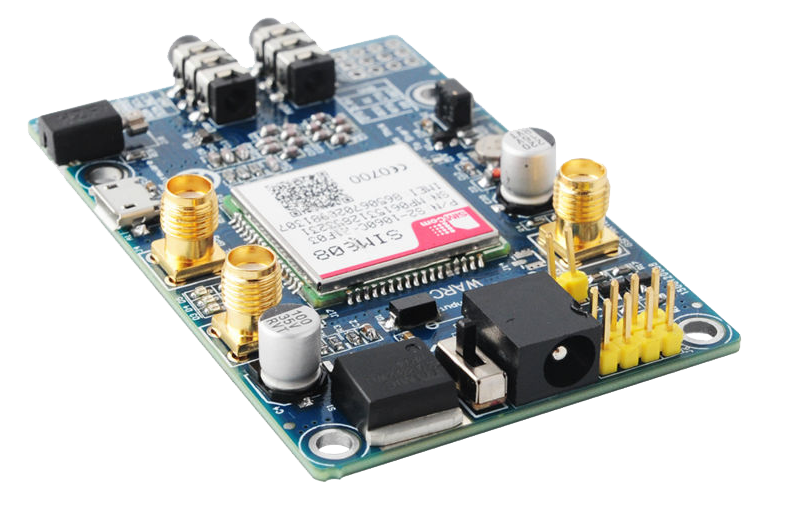
\includegraphics[width=0.5\textwidth]{images/gprs.png}
\caption{Komunikační modul GSM/GPRS - SIM808}
\label{image}
\end{center}
\end{figure}

\section{Desktopová aplikace}
Na základě požadovaných vlastností jsem cílový operační systém jsem zvolil Windows 10, jakožto v evropě nejrozšířenější \cite{DesktopMarketShare}. Programovací jazyk C\# a vývojové prostředí Visual Studio 2017. Jednotlivé požadavky kladené na desktopovou aplikaci lze nalézt níže. Komunikace s aplikací bude probíhat skrze připojení USB (COM).

\section{Mobilní aplikace}
Cílový operační systém jsem zvolil Android, jakožto v evropě nerozšířenější \cite{MobileMarketShare}. Programovací jazyk Java a vývojové prostředí a Android Studio. Jednotlivé požadavky kladené na mobilní aplikaci lze nalézt níže. Komunikace bude probíhat skrze mobilní datovou síť.

\section{Webová aplikace}
Not implemented yet.

\section{Komunikační server}
Pperační systém jsem zvolil Windows 10, kvůli rychlosti vývoje. Programovací jazyk C\# a vývojové prostředí Visual Studio 2017. Komunikace s aplikací bude probíhat skrze pevné připojení k internetu.

% Domovní systém (hardware a firmware)

\chapter{Domovní systém}

\section{Slepá cesta vývoje (využití mobilního telefonu)}
Následující část pojednává o snaze využít GSM/GPRS modulu integrovaném v „hloupém“ mobilním telefonu. Práce na této části zabrali přibližně dva měsíce, po kterých se tato cesta ukázala jak slepá, proto byla zavrhnuta.

\subsection{Využití mobilního telefonu pro datovou komunikaci}
Jednou z prvních myšlenek této práce bylo, zdali je možné využít starší „hloupý“ mobilní telefon pro přístup do datové sítě. V aktuální době se mobilní telefony rozdělují do dvou hlavních kategorií, tedy chytré telefony a klasické "hloupé" telefony.

U chytrých telefonů je získání přístupu do sítě GPRS triviální. Stačí napsat software, který tyto zdroje poskytne přes port USB a tím je problém vyřešen. Klasické telefony se dělí do dvou podkategorií. 

První podkategorie jsou telefony s dokumentací a s API. Některé starší telefony měli otevřené dokumentace a některá dokonce i API přímo pro tyto účely (Motorola, Nokia). Pro tyto mobilní telefony existuje velké množtví návodů a postupů, jak připojení do sítě GPRS docílit. 

Druhou podkategorií jsou mobilní telefony bez otevřených dokumentací a bez API, která by zpřístupňovala zdroje mobilního telefonu. Pro tyto mobilní telefony jsem nenalezl žádné dostupné řešení, přitom jsou to telefony nejrozšířenější, tím se staly pro tento projekt zajímavými.

\paragraph{Získání přístupu do sítě GPRS, skrze:}
\begin{itemize}
\item Chytrý telefon (vyřešeno)
\item Klasický telefon s API (vyřešeno)
\item Klasický telefon bez API a dokumentace (nevyřešeno)
\end{itemize} 

\subsection{Klasický telefon bez API a dokumentace}
Prvním úkolem bylo vybrání vhodného telefonu pro tyto účely. Po provedení průzkumu trhu jsem zjistil, že je možné vybírat jak z bazarových kusů, tak z nových. Zajímavým zjištěním bylo, že ceny nových telefonů podporujících s funkcí GSM i GPRS se pohybují kolem 450 Kč s DPH za kus. Bazarové kousky začínají na 600 Kč s DPH za kus. Vzhledem k nižší ceně, záruce a garanci funkčnosti jsem se rozhodl zakoupit nový model.

\subsection{Tlačítkový telefon STK R45i}
Při výběru nového telefonu jsem primárně sledoval cenu a přítomnost GPRS. Bezkonkurenčně nejlevnějším telefonem byl tlačítkový mobil od britského výrobce STK R45i. Zakoupen byl prostřednictvím internetového obchodu Alza.cz za cenu 419 Kč s DPH bez dopravy. Cena s dopravou činila celkových 449 Kč s DPH.

Před obdržením zakoupeného telefonu jsem provedl průzkum, zda existují dokumentace, nebo zda se pokoušel někdo o něco podobného u této značky. Kromě oficiálního letáku s velice obecnými parametry přístroje jsem nenalezl žádné veřejné dokumentace. Stejně tak jsem nenalezl žádné informace o tom, že by někdo prováděl, třeba i rozbor, tohoto, či jiného zařízení od této značky. Ihned po obdržení jsem se tedy pustil do vlastního průzkumu.

\begin{figure}[H]
\begin{center}
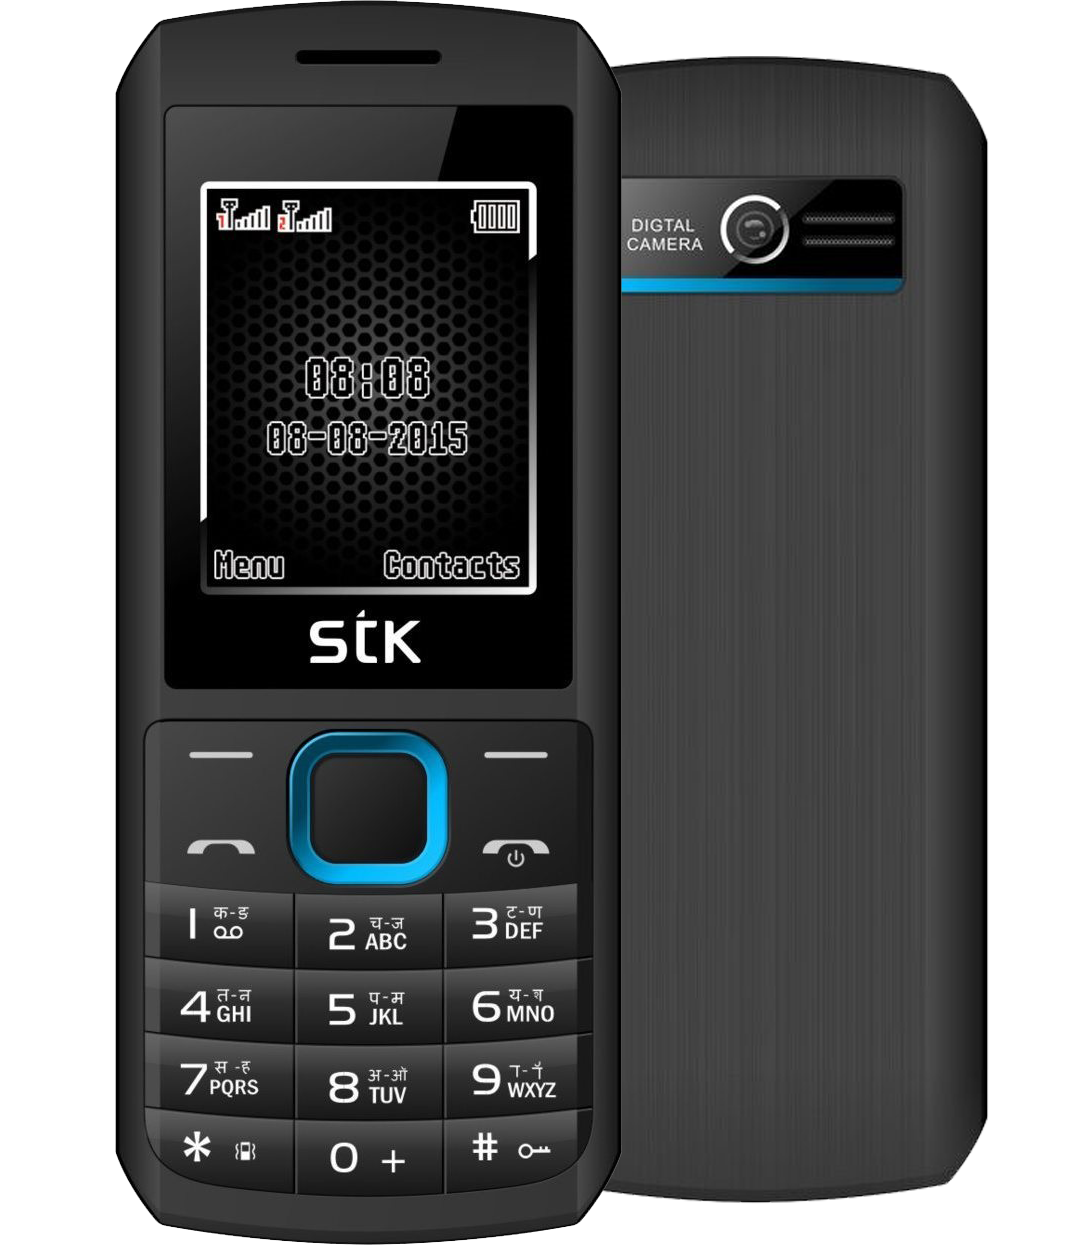
\includegraphics[width=0.4\textwidth]{images/phone.png}
\caption{Zakoupený mobilní telefon STK R45i}
\label{image}
\end{center}
\end{figure}

\subsection{Kontaktování výrobce}
Bez existujících dokumentací jsem se nejdříve rozhodl kontaktovat samotného výrobce s vysvětlením mého projektu a žádostí o poskytnutí dokumentačních podkladů. Napsal jsem celkem na 3 oddělení britské společnosti, přesněji na obchodní, podporu a servis. Do jednoho týdne přišla shodná odpověď od všech tří kontaktovaných oddělení. Zprávou bylo, že mi dokumentace neposkytnou a že mi v mé práci nemohou pomoci.

\begin{figure}[H]
\begin{center}

\includegraphics[width=0.6\textwidth]{images/response.png}
\caption{Jedna z odpovědí od společnosti STK}
\label{image}
\end{center}
\end{figure}

\subsection{Rozebrání mobilního telefonu}
Vzhledem k negativní odpovědi výrobce jsem zahájil vlastní výzkum. Prvním pokusem byla komunikace s mobilním telefonem skrze USB, stejně jako to bylo možné u telefonů s API k těmto účelům. Několik týdnů výzkumu jsem zasvětil pokusům o přímou komunikaci po seriové lince. Bez úspěchu.

Po dohodě s vedoucím práce, jsem se rozhodl porušit záruku a rozebrat telfefon. Zaměřil jsem se primárně na případné servisní piny pro připojení a diagnostiku. Po hlubším prozkoumání se mi podařilo nalézt servisní piny, které jsem se následně snažil analyzovat a skrze ně komunikovat s mobilním telefonem. Po několika týdnech opět bez úspěchu.

\begin{figure}[H]
\begin{center}
\includegraphics[width=0.7\textwidth]{images/servicePins.png}
\caption{Servisní piny}
\label{image}
\end{center}
\end{figure}

\subsection{Závěr rozboru}
Po dvou měsíčním snažení se z mobilního telefonu nepodařilo získat žádnou informaci. První týden se mi podařilo zachytávat neznámé signály, nicméně po hlubším přezkoumání spektrálním analyzátorem bylo zjištěno, že se nejedná o číslicový signál. Tuto cestu jsem byl nucen uzavřít a oznámit vedoucímu, že tudy cesta nevede. Od využití mobilního telefonu bylo tedy upuštěno a jako vstupní brána do GPRS byl pořízen samostatný GSM/GPRS modul.

\section{Prototyp domovního systému}
Účelem prototypu je vývoj a testování firmware a vzájemné komunikace s jednotlivými aplikacemi. Zapojení musí být modulární, snadno přepojitelné a jednoduše přístupné k měření.

\subsection{Blokové schéma}
Prototyp je rozdělen do třech hlavních bloků, které spolu vzájemně komunikují. Pod blokovým schématem následuje detailní popis těchto jednotlivých částí.

\begin{figure}[H]
\begin{center}
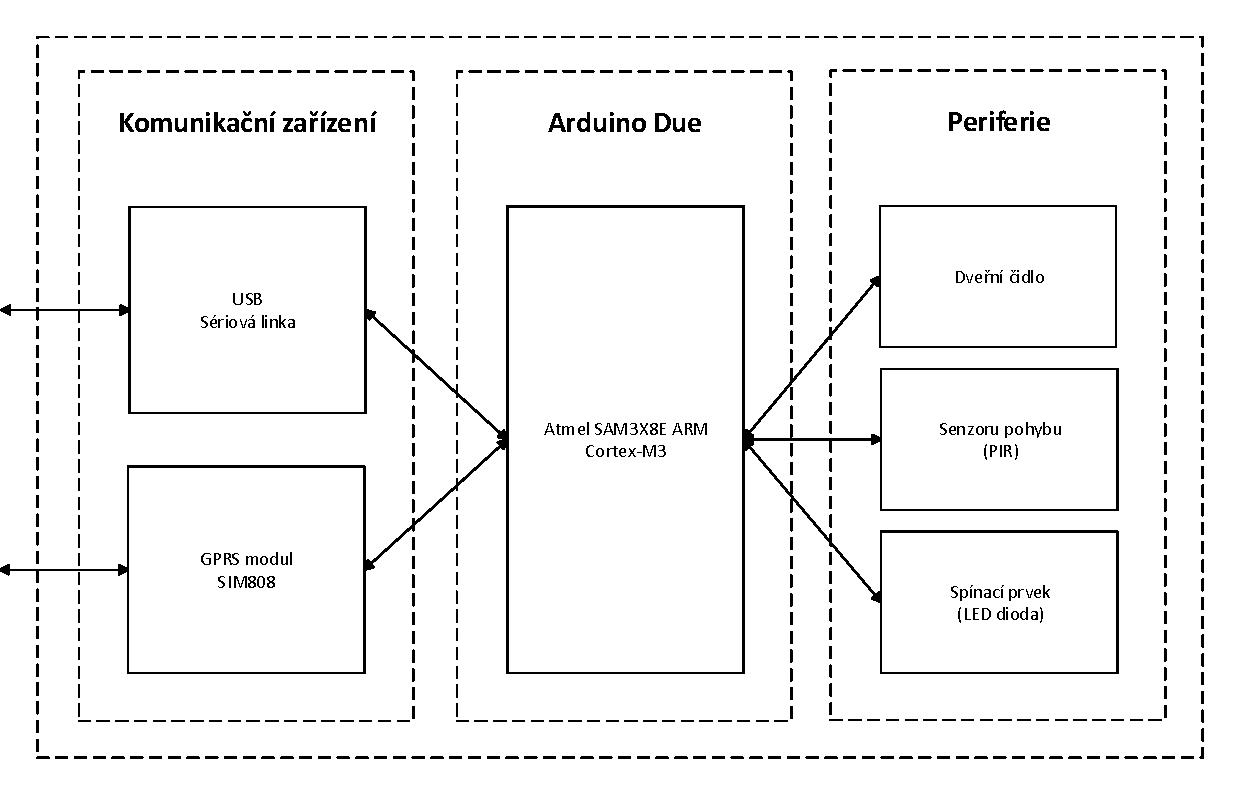
\includegraphics[width=\textwidth]{vector/blokoveSchemaHardware.pdf}
\caption{Blokové schéma zapojení prototypu domovního systému}
\label{image}
\end{center}
\end{figure}

\paragraph{Komunikační zařízení:}
Blok „Komunikační zařízení“ obsahuje všechna zařízení zprostředkovávající komunikaci. Vždy potřebujeme komunikovat pomocí USB a internetového připojení. V případě prototypu složí k USB komunikaci vestavěn řadič USU, který se nachází na desce Arduino. Internetové připojení zprostředkovává GPRS modul, v případě prototypu model SIM808, případně podobný.

\paragraph{Arduino Due:}
Hlavní blok „Arduino Due“ obsahuje vývojvou desku Arduino Due, která slouží jako centrální jednotka celého domovního systému. Do této jednotky jsou zapojeny veškeré periferie, ať již komunikátory, nebo senzory a spínače.

\paragraph{Periferie}
Blok „Periferi“ obsahuje všechna čidla, senzory, spínače a podobná zařízení, které má za úkol řídící jednotka kontrolovat. Pro demonstraci základních funkcionalit jsem zvolil dveřní čidlo, senzor pohybu PIR a spínací prvek typu LED dioda. Všechny tyto periferie lze jednodšue nahradit jinou libovolnou součástkou, případě nové přidat.

\subsection{Výsledný prototyp}
Výsledný prototyp je schopen simulovat reálné nasazení domovnío systému. Obsahuje řídící desku Arduino, GSM modul pro připojení do sítě internet, jeden spínací prvek (LED) a dva senzory diody (PIR a dveřní čidlo). Každý senzor má svou vlastní kontrolní diodu. Ta signalizuje, zda je senzor sepnutý či nikoliv.

\begin{figure}[H]
\begin{center}
\includegraphics[width=\textwidth]{images/board.png}
\caption{Finální prototyp na nepájivém poli}
\label{image}
\end{center}
\end{figure}

\subsection{Schéma zapojení}
Not implemented yet.

\section{Firmware}
Hlavním účelem firmware (software pro řídící jednotku) je možnost kompletního řízení domovního systému a umožnění komunikace, včetně poskytování API pro přístup aplikací. Software byl vyvinut pro platformu Arduino (čip ARM Cortex-M3) v programovacím jazyce C++ s nadstavbou Wiring (knihovna pro řízení hardwaru) \cite{Wiring}, za pomocí vývojového prostředí Visual Studio 2017 s rozšířením Visual Micro \cite{Visual Micro}, které poskytuje zvýrazňování syntaxe knihovny Wiring a umožňuje komplikaci a nahrávání kódu přímo na desku Arduino.

Dále budou zmíněny pouze ty části, které jsou důležité pro pochopení nastavení zařízení a přístupu k aplikaci (API), samotný kód lze nalézt v příloze a zmiňován zde nebude.

\subsection{Nastavení}
Inicializační část slouží k prvotnímu nastavení mikrokontroleru před spuštěním. Toto nastavení lze měnit pouze před první kompilací kódu, za běhu programu jej změnit nelze. Jedinou cestou k jeho změně je tedy opětovná kompilace kódu s upraveným nastavením a následné nahrání do mikrokontroleru.

\paragraph{Nastavit lze:}
\begin{itemize}
\item Komunikační rychlost (baudRate)
\item Maximální počet senzorů
\item Maximální počet spínačů
\item Kódy chybových hlášek
\item Klíčová slova API
\end{itemize} 

\subsection{API}
Funkce API jsou nazvány podle své činnosti. Při volání jednolivých funkcí se posílá nejdříve název funkce, které následují kulaté závorky, tedy \uv{(} a \uv{)}, vnichž jsou uvedeny jednotlivé parametry. Každý jeden parametr je oddělen čárkou. Ve výsledku může výstup vypadat například takto \uv{SetSensor(10,5)}. V následující tabulce jsou vypsány všechny dostupné funkce, typu getter.

\renewcommand{\arraystretch}{1.5}
\begin{table}[H]
\begin{center}
\begin{tabular}{| l | c | c| c |}
\hline
Funkce & Parametry & Popis & Vrací\\
\hline
\hline
GetAllSensors() & / & Vrací list všech senzorů & id, pin, name, state \\
\hline
GetAllSwitches() & / & Vrací list všech spínačů & id, pin, name, state \\
\hline
\end{tabular}
\end{center}
\caption{Tabulka API - Getters}
\end{table}

\paragraph{Ukázka vrácených senzorů:}
\begin{center}
Sensors((Id = 0,Pin = 8,Name = Door Sensor,State = 0,Type = 0)(Id = 1,Pin = 7,Name = PIR Sensor,State = 0,Type = 1))
\end{center} 

\paragraph{Ukázka vrácených spínačů:}
\begin{center}
Switches((Id = 0,Pin = 6,Name = Led Switch,State = 0))
\end{center} 

Další tabulka obsahuje výpis všech dostupných funkcí, typu setter.

\renewcommand{\arraystretch}{1.5}
\begin{table}[H]
\begin{center}
\begin{tabular}{| l | c | c| c |}
\hline
Dotaz & Parametry & Popis & Vrací\\
\hline
\hline
SetSensorName() & id, name & Změna jména senzoru & OK, ERROR \\
\hline
SetSwitchName() & id, name & Změna jména spínače & OK, ERROR \\
\hline
SetSensorPin() & id, pin & Změna pinu senzoru & OK, ERROR \\
\hline
SetSwitchPin() & id, pin & Změna pinu spínače & OK, ERROR \\
\hline
SetSensorType() & id, type & Změna typu senzoru & OK, ERROR \\
\hline
SetSwitchState() & id, state & Změna stavu spínače & OK, ERROR \\
\hline
AddSensor() & pin, name, type & Přidání nového senzoru & OK, ERROR \\
\hline
AddSwitch() & pin, name, state & Přidání nového spínače & OK, ERROR \\
\hline
DeleteSensor() & id & Smazání senzoru & OK, ERROR \\
\hline
DeleteSwitch() & id & Smazání spínače & OK, ERROR \\
\hline
\end{tabular}
\end{center}
\caption{Tabulka API - Setters}
\end{table}

U nastavovacích dotazů musí být \uv{id} a \uv{pin} číslo od 0 do 100, \uv{type} a \uv{state} musí být číselné hodnoty 0 (false) nebo 1 (true) a \uv{name} musí být maximálně 30 znaků dlouhé (30 bytů). Pro \uv{state} znamená 1 zapnuto, 0 vypnuto. Pro \uv{type} znamená 1 \uv{normálně vypnuto / push to make} a 0 \uv{normálně zapnuto / push to break}. Pokud jedna z podmínek nebude splněna, dotaz bude odmítnut. Parametr \uv{ID} lze získat pomocí příkazu \uv{GetAllSensors()} a \uv{GetAllSwitches} z již existujících zařízení.

\paragraph{Ukázka přidání nového senzoru:}
\begin{center}
AddSensor(8, Muj novy senzor, 0)
\end{center}

\paragraph{Ukázka změny pinu senzoru:}
\begin{center}
SetSensorName(1, Moje nove jmeno senzoru)
\end{center}

\paragraph{Ukázka smazání spínače:}
\begin{center}
DeleteSwitch(1)
\end{center}

\subsection{Notifikace}
Řídící jednotka má uložené všechny poslední stavy senzorů a při každém průchodu hlavní smyčkou proběhne čtení, pomocí funkce \uv{checkSensorStateChangedAndSendIfTrue()}. Pokud nový stav nesouhlasí se starým, je zaslána notifikace s ID zařízení a aktuálním stavem. Poté záleží na cílové aplikaci, jak informaci zpracuje.

\paragraph{Ukázka notifikace:}
\begin{center}
Sensor(Id = 1,State = 0)
\end{center} 

\subsection{Chybová hlášení}
Chybová hlášení (při neúspěšném provedení operace nebo jiné chybě) byla původně tvořena pomocí stavových kódů HTML \cite{HTML1.1}. Z důvodu nedostatku paměti (při vvoji na platformě Arduino Uno) byla nahrazena jednoduchým \uv{OK} a \uv{ERROR}. Kontrola chyb se provádí vždy při zpracovávání kterékoliv z operací podporující API. Vždy se kontroluje, zda je možné zapsat, zda se provedl zápis, zda je nová hodnota po přečtení stejná jako zapisovaná, a tak dále. Pokud nastane chyba, je vše vráceno do původního stavu. Pokud příkaz nebyl rozpoznán, nebo nesplňuje kritéria tohoto API, je vrácena chybová hláška o nerozpoznání příkazu.
\paragraph{Ukázka odpovědi při nerozpoznání příkazu:}
\begin{center}
Command 'SetSensor(15,5)' not recognized.
\end{center} 

% Desktopová aplikace

\chapter{Desktopová aplikace}
Hlavním účelem desktopové aplikace je možnost kompletního nastavení a monitorování zabezpečovacího zařízení. Aplikace se zaměřuje zejména na správu (vytváření, upravování, mazání) všech senzorů a spínačů. Software byl vyvinut pro operační systém Windows v programovacím jazyce C\#, za pomocí IDE Visual Studio 2017. Design byl inspirovaný manuálem jednotného vizuálního stylu TUL \cite{TULVisual}.

\section{Blokové schéma}
Kód aplikace je rozdělen do třech hlavních bloků, které spolu vzájemně komunikují. Pod blokovým schématem následuje detailní popis těchto jednotlivých částí.

\begin{figure}[H]
\begin{center}
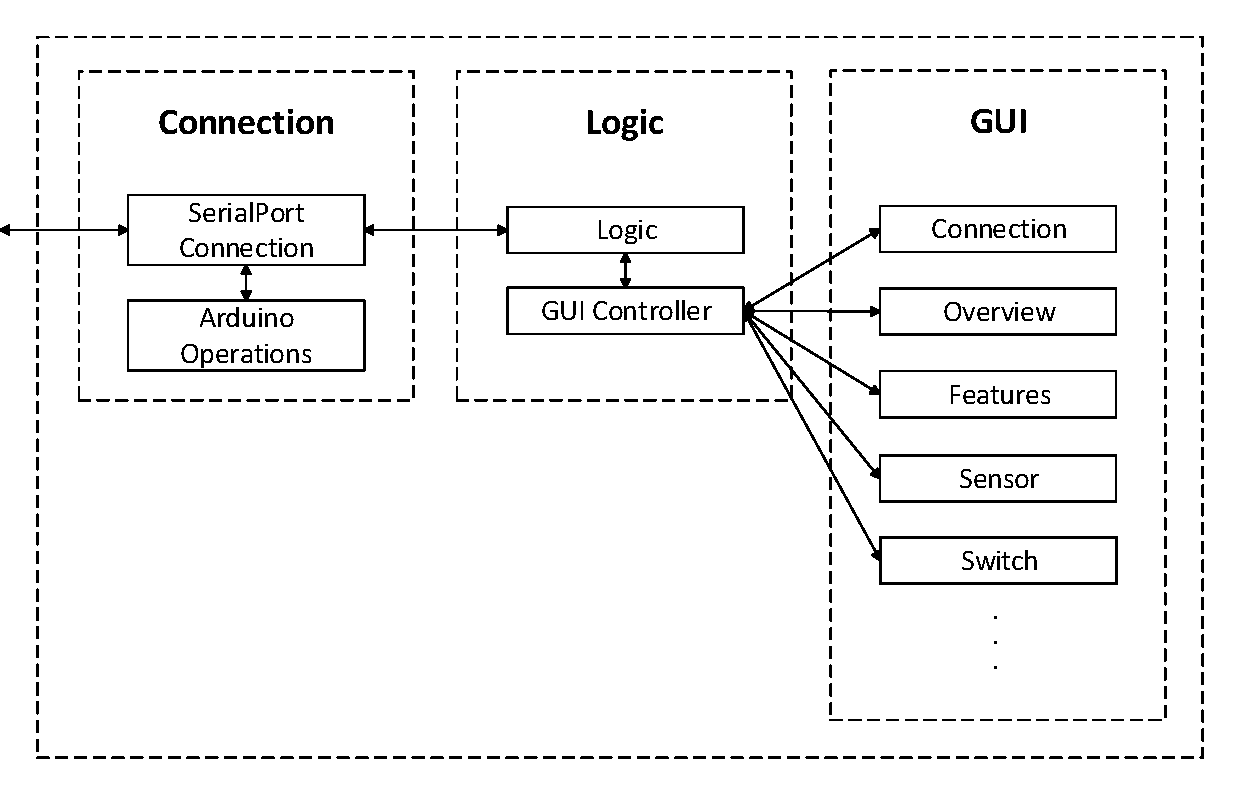
\includegraphics[width=\textwidth]{vector/blokoveSchemaSecurityControl.pdf}
\caption{Blokové schéma objektového návrhu aplikace}
\label{image}
\end{center}
\end{figure}

\subsection{Connection}
Blok „Connection“ slouží k připojení řídící jednotky skrze seriovou linku (SerialPort Connection), po které komunikuje za pomocí API, poskytované touto jednotkou. Po navázání spojení se určí typ připojené řídící jednotky, kvůli poskytnutí seznamu použitelných pinů. Výstupem tohoto bloku jsou funkce pro jednoduché zapisování a čtení z této jednotky (Arduino Operations), včetně kompletního seznamu použitelných pinů této jednotky. Seznam podporovaných řídících jednotek Arduino lze nalézt v části Kompatibilita.

\subsection{Logic}
Blok „Logic“ je hlavní vlákno, které načítá veškeré viditelné části aplikace (GUI Controller) z bloku „GUI“ a zároveň zprostředkovává komunikaci mezi blokem Connection a jednotlivými funkcemi v oknech aplikace (GUI). Nachází se zde tedy napojení na Arduino Operations z bloku „Connection“. Zároveň zpracovává všechny informace, přicházejících směrem od řídící jednotky (například notifikace, chybová hlášení, stavové kódy atd.).

\subsection{GUI}
Blok „GUI“ poskytuje jednotlivé funkce aplikace, včetně jejich grafického uživatelského rozhraní. Například „Overview“ poskytuje GUI pro přehled všech připojených senzorů a spínačů, „Senzor“ poskytuje GUI pro vytváření a upravování senzorů. Tyto funkce jsou využívány v bloku „Logic“, za pomocí „GUI Controlleru“, který je načítá do hlavního okna aplikace.

\section{Grafické uživatelské rozhraní}
V této části textu budou zmíněny pouze ty části GUI, které jsou důležité pro pochopení ovládání aplikace.

\subsection{Připojení/odpojení řídící jednotky (Connection)}

\begin{figure}[H]
\begin{center}
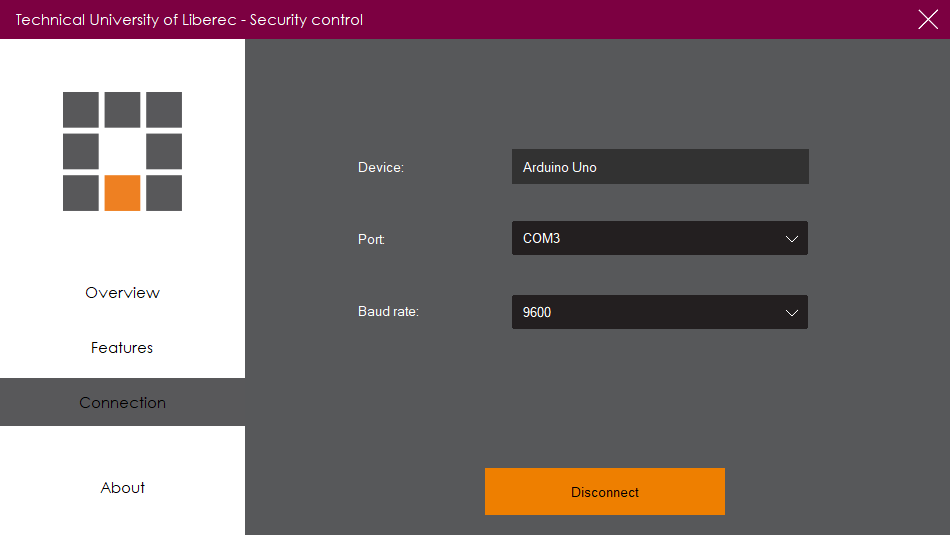
\includegraphics[width=\textwidth]{images/connection.png}
\caption{Okno s možností připojení/odpojení řídící jednotky}
\label{image}
\end{center}
\end{figure}

Záložka „Connection“ slouží k připojení či odpojení řídící jednotky. Tato záložka hlídá, zda je připojení stále aktivní. Při ztrátě spojení ihned informuje uživatele a upraví chování celé aplikace. Záložka rovněž hlídá, zda se neobjevilo nové zařízení k připojení, pokud ano, informuje uživatele a zobrazí nově dostupná zařízení. 

Zařízení pro připojení se vybírá pomocí „Port“, které obsahuje seznam všech dostupných COM portů. K vybranému COM portu je následně zjištěn název zařízení, který se objeví v „Device“. Rychlost komunikace (BaudRate), lze vybrat ze standardních komunikačních rychlostí \cite{BaudRates}. Vybraná komunikační rychlost musí být stejná, jako v řídící jednotce. Automaticky nastavená hodnota 9600 by měla odpovídat přednastavené rychlosti řídící jednotky. 

Po zvolení řídící jednotky a komunikační rychlosti stačí zmáčknou oranžové tlačítko „Connect“ pro připojení, případně „Disconnect“ pro odpojení.  

\paragraph{Dostupné komunikační rychlosti (BaudRate):}
\begin{itemize}
\item 300, 600, 1200, 2400, 4800, 9600, 14400, 19200, 28800, 38400, 57600, 115200
\end{itemize} 

\subsection{Přehled připojených komponent (Overview)}

\begin{figure}[H]
\begin{center}
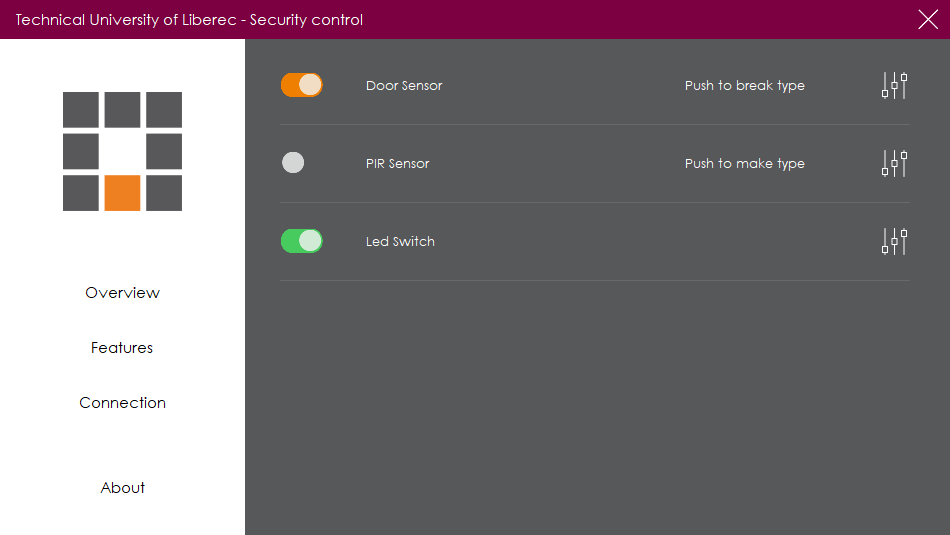
\includegraphics[width=\textwidth]{images/overview.png}
\caption{Okno s přehledem jednotlivých komponent}
\label{image}
\end{center}
\end{figure}

Přehled připojených komponent (Overview) slouží pro zobrazení všech dostupných spínačů a senzorů, které jsou v řídící jednotce dostupné. Obsah se generuje dynamicky pod sebe, lze tedy zobrazit neomezený počet zařízení (po přetečení viditelné části se objeví scrollbar). Každý dynamický řádek je zobrazen dle svého typu, tedy zda se jedná o senzor nebo spínač. U spínačů lze měnit jejich aktuální stav, u senzorů lze aktuální stav pouze sledovat. V obou případech lze měnit interní nastavení každého zařízení, pomocí tlačítka na pravé straně. V případě, že žádná zařízení neexistují, je uživatel upozorněn. 

Žádná data nejsou editována v objektech uvnitř aplikace, ale žádosti o změnu jsou zasílány do řídící jednotky. Po obdržení odpovědi se buď projeví požadovaná změna, nebo je zobrazeno chybové hlášení. V obou případech je uživatel je upozorněn zda změna proběhla, či zda neproběhla.

\subsection{Nastavení senzoru (Sensor Edit)}

\begin{figure}[H]
\begin{center}

\includegraphics[width=\textwidth]{images/settings.png}
\caption{Okno s nastavením senzoru}
\label{image}
\end{center}
\end{figure}

Nastavení senzoru slouží k změně interního nastavení uvnitř řídící jednotky. Lze měnit název zařízení (omezeno na 30 znaků), pin na kterém se senzor nachází, typ senzoru (rozpínací, spínací) a poslední možností je smazání senzoru. Výběr pinů závisí vždy na připojené desce. Pro tento účel byl vytvořen kompletní seznam všech testovaných a kompatibilních desek, které lze k softwaru připojit. Kompletní seznam desek, které lze použít, je k nalezení v části textu nazvané „Podporované řídící jednotky“. 

Žádná data nejsou editována v objektech uvnitř aplikace, ale žádosti o změnu jsou zasílány do řídící jednotky. Po obdržení odpovědi se buď projeví požadovaná změna, nebo je zobrazeno chybové hlášení. V obou případech je uživatel je upozorněn zda změna proběhla, či zda neproběhla.

\subsection{Nastavení spínače (Switch Edit)}
Nastavení je téměř identické s předchozím, proto není nutné náhledový obrázek. Lze měnit název (omezeno na 30 znaků), pin na kterém se spínač nachází. Jedinou změnou možnost změny stavu tohoto spínače (zapnuto/vypnuto).

Žádná data nejsou editována v objektech uvnitř aplikace, ale žádosti o změnu jsou zasílány do řídící jednotky. Po obdržení odpovědi se buď projeví požadovaná změna, nebo je zobrazeno chybové hlášení. V obou případech je uživatel je upozorněn zda změna proběhla, či zda neproběhla.

\subsection{Možnosti programu (Features)}
Tato záložka zpřístupňuje různá nastavení a funkce, které nejsou běžně potřebné.

\paragraph{Přehled funkcí:}
\begin{itemize}
\item Přidat nový senzor
\item Přidat nový spínač
\item Znovu načíst všechna data z řídící jednotky
\item Zobrazovat notifikace, pokud se změní stav senzoru (přepínač)
\item Zobrazovat notifikace, pokud se senzor navrátí do výchozího stavu (přepínač)
\end{itemize} 

\subsection{Notifikace}
Aplikace podporuje širokou škálu notifikací, upozornění a varovných hlášení, která slouží pro upozornění uživatele na nastalou situaci. Například se jedná o změnu stavu pinů, chybové stavy řídící jednotky, nebo odpojení zařízení. Notifikace se zachytávají v hlavním okně, v části kódu nazvané \uv{Autocalled functions (Events from Arduino)}, pomocí eventů.

\paragraph{Přehled implementovaných notifikací:}
\begin{itemize}
\item Připojení zabezpečovacího zařízení
\item Odpojení zabezpečovacího zařízení
\item Ztráta spojení zabezpečovacího zařízení
\item Automatický pokus o připojení se nezdařil
\item Stav spínače přenastaven
\item Stav senzoru se změnil
\item Interní chyba řídící jednotky
\item Jméno se podařilo/nepodařilo změnit
\item PIN se podařilo/nepodařilo změnit
\item Typ senzoru se podařilo/nepodařilo změnit
\item Nový senzor se podařilo/nepodařilo přidat
\item Nový spínač se podařilo/nepodařilo přidat
\item Komponenty arduina se podařilo/nepodařilo znovu načíst
\item Nastavení notifikací změněno
\end{itemize} 

\section{Kompatibilita}

\subsection{Testované verze Windows 10}
Desktopová aplikace byla testována pod operačním systémem Windows 10 ve všech (v době psaní práce) vydaných sestavách a pro tento systém byla také optimalizována. Nicméně cílová platforma Microsoft .NET Framework 4.5.2 \cite{WhatsNew.NetFramework4.5.2} by měla zajišťovat zpětnou kompatibilitu až do systému Windows Vista. Jmenovitě pro Windows Vista SP2, Windows 7 SP1, Windows 8, Windows 8.1, Windows 10 a novější \cite{.NetFramework4.5.2}.

\paragraph{Seznam všech testovaných sestav systému Windows 10:}
\begin{itemize}
\item Version 1507 - Build 10.0.10240 (čistá instalace systému)
\item Version 1511 - Build 10.0.10586 (November Update)
\item Version 1607 - Build 10.0.14393 (Anniversary Update)
\item Version 1703 - Build 10.0.15063 (Creators Update)
\item Version 1709 - Build 10.0.16299 (Fall Creators Update)
\item Version 1803 - Build 10.0.17134 (April 2018 Update)
\end{itemize}

\subsection{Podporované řídící jednotky}
Řídící jednotka, v případě tohoto prototypu deska Arduino, existuje v několika variantách \cite{ArduinoProducts}. Jako řídící jednotku je vhodné použít jednu z řady produktů ENHANCED FEATURES (Mega, Due a další) \cite{ArduinoProducts}, vzhedem k tomu, že obsahují dostatečné množství paměti \cite{CompareBoardSpecs} pro udržování většího množství senzorů a spínačů. Vybrané jednotky, které jsou pro tento projekt použitelné, jsem otestoval a zařadil mezi jednotky podporované. Tyto podporované jednotky se vyznačují tím, že desktopová aplikace obsahuje seznam použitelných pinů pro každou z těchto desek. Tento seznam se získává ihned po připojení jednotky, a to na základě názvu desky poskytnutého řadičem. Pokud připojená deska není v seznamu, použije se seznam pinů pro desku Arduino Uno. V takovémto případě není zaručena správná funkčnost softwaru. Pokud použitý pin není v seznamu pinů desky, zařízení na tomto pinu nebude možné ovládat, upravovat, ani s ním jakkoliv pracovat.

\paragraph{Seznam všech podporovaných řídících jednotek:}
\begin{itemize}
\item Arduino/Genuino Uno (nedoporučeno)
\item Arduino/Genuino Mega
\item Arduino/Genuino Mega 2560
\item Arduino Due (doporučeno)
\end{itemize}

\paragraph{Seznam desek kompatibilních s Arduino/Genuino Uno:}
\begin{itemize}
\item Arduino/Genuino Duemilanove
\item Arduino/Genuino Diecimila
\item Arduino/Genuino Nano
\item Arduino/Genuino NG
\item Arduino/Genuino Mini
\item Arduino/Genuino Extreme
\item Arduino/Genuino USB
\item Arduino/Genuino Serial
\item Arduino/Genuino 101
\end{itemize}

% Mobilní aplikace

\chapter{Mobilní aplikace}
Hlavním účelem mobilní aplikace je čisté monitorování řídící jednotky. Není tedy možno měnit jakékoliv nastavení (k čemuž slouží desktopová aplikace). Tato aplikace byla vyvinuta pro mobilní operační systém Android 4.0.3 (Ice Cream Sandwich - API 15) a vyšší, v programovacím jazyce Java, za pomocí IDE Android Studio 2.3.2. Design byl inspirovaný manuálem jednotného vizuálního stylu TUL \cite{TULVisual}.

\section{Blokové schéma}
Kód aplikace je rozdělen do třech hlavních bloků, které spolu vzájemně komunikují. Pod blokovým schématem následuje detailní popis těchto jednotlivých částí.

\begin{figure}[H]
\begin{center}
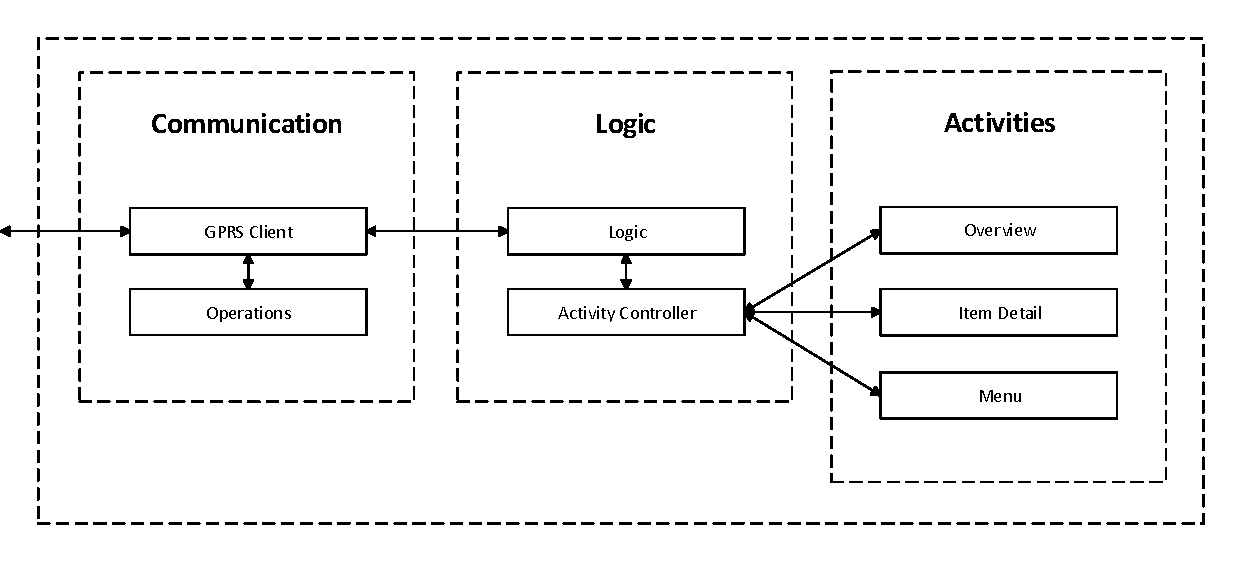
\includegraphics[width=\textwidth]{vector/blokoveSchemaSecurityViewer.pdf}
\caption{Blokové schéma objektového návrhu aplikace}
\label{image}
\end{center}
\end{figure}

\subsection{Communication}
Blok „Communication“ slouží k připojení řídící jednotky skrze internetové připojení (GPRS), za pomocí mobilní datové sítě. Toto připojení komunikuje pomocí API, poskytované řídící jednotkou. Po navázání spojení se zažádá o všechna dostupná data, která může řídící jednotka poskytnout. Samotnou komunikaci zpracovává vlákno „GPRS Client“, které je napojené na „Operations“, kde se nachází implementace API.

Aby internetová komunikace fungovala, musel být napsán komunikační server, který je pevným bodem v síti. Server na dané IP adrese a portu, zajišťuje komunikaci všech existujících řídících jednotek a mobilních aplikací. Více o této problematice v části textu nazvané „Komunikační server“.

\subsection{Logic}
Blok „Logic“ je hlavní vlákno, které díky „Activity Controlleru“ načítá veškeré viditelné části aplikace z bloku „Activities“ a zároveň zprostředkovává komunikaci mezi blokem Communication a jednotlivými funkcemi v oknech aplikace (Activities). Nachází se zde tedy napojení na Arduino Operations z bloku „Communication“. Zároveň zpracovává všechny informace, přicházejících směrem od řídící jednotky (například notifikace, chybová hlášení, stavové kódy atd.).

\subsection{Activities}
Blok „Activites“ poskytuje jednotlivé funkce aplikace, včetně jejich GUI, v Androidu nazvaném jako Activity. Například „Overview“ poskytuje Activity pro přehled všech připojených senzorů a spínačů, „Item Detail“ poskytuje Activity přehled o všech dostupných informací, které o vybrané komponentě aplikace má, a „Menu“ poskytuje Acitivity s nastavením. Tyto funkce jsou využívány v bloku „Logic“, za pomocí „Activity Controlleru“, který je načítá do hlavního okna aplikace.

\section{Grafické uživatelské rozhraní}
V této části textu budou zmíněny pouze ty části GUI (Activities), které jsou důležité pro pochopení ovládání aplikace.

\subsection{Přehled připojených komponent}
\begin{figure}[H]
\begin{center}
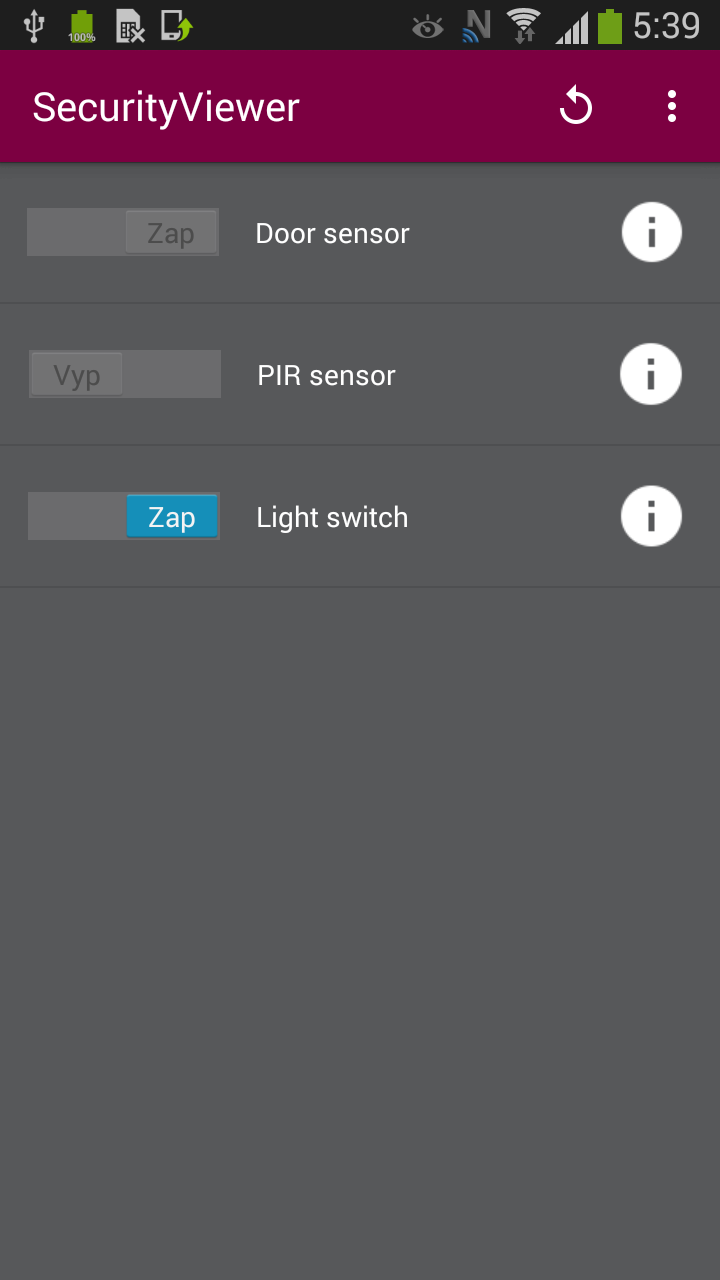
\includegraphics[width=0.4\textwidth]{images/app1.png}
\caption{Okno s přehledem jednotlivých komponent}
\label{image}
\end{center}
\end{figure}

Stejně jako v případě desktopové aplikace, slouží přehled připojených zařízení pro zobrazení všech dostupných spínačů a senzorů, které jsou v řídící jednotce dostupné. Obsah se generuje dynamicky pod sebe, lze tedy zobrazit neomezený počet zařízení (po přetečení viditelné části se objeví scrollbar). Každý dynamický řádek je zobrazen dle svého typu, tedy zda se jedná o senzor nebo spínač. U spínačů lze měnit jejich aktuální stav, u senzorů lze aktuální stav pouze sledovat. V obou případech lze zobrazit interní nastavení každého zařízení, pomocí tlačítka na pravé straně. V případě, že žádná zařízení neexistují, je uživatel upozorněn.

Tlačítko na pravé straně „i“, tedy značí zobrazení podrobností vybrané komponenty. Dále v horní liště vidíme zatočenou šipku, která značí ruční aktualizaci všech zařízení. Posledním prvkem horního menu jsou tři tečky, takzvané „Hamburger Menu“, které složí pro otevření nastavení aplikace.

Žádná data nejsou editována v objektech uvnitř aplikace, ale žádosti o změnu jsou zasílány do řídící jednotky. Po obdržení odpovědi se buď projeví požadovaná změna, nebo je zobrazeno chybové hlášení. V obou případech je uživatel je upozorněn zda změna proběhla, či zda neproběhla.

\subsection{Podrobnosti vybrané komponenty}
\begin{figure}[H]
\begin{center}
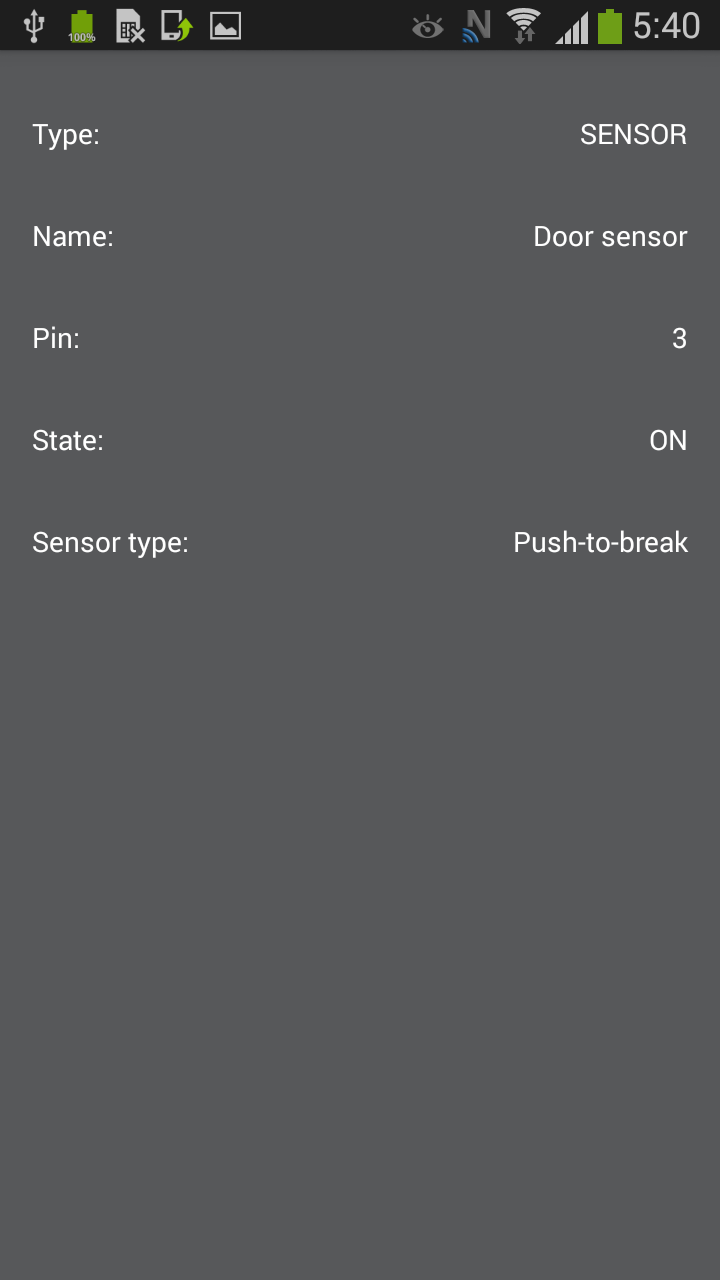
\includegraphics[width=0.4\textwidth]{images/app2.png}
\caption{Detailní přehled nastavení komponenty}
\label{image}
\end{center}
\end{figure}

Zobrazení podrobností o vybrané komponentě ukazuje všechny dostupné údaje, které má aplikace k dispozici. Běžně se tak jedná o typ zařízení (senzor, spínač), název zařízení (omezeno na 30 znaků), číslo pinu, na kterém je zařízení připojení, a stav zařízení (zapnuto, vypnuto). Pokud se jedná o senzor, je zde vyobrazen i typ vybraného senzoru (spínací, rozpínací).

Vrátit se lze tlačítkem zpět, které má každý mobilní telefon se systémem Android implementované (ať již softwarově nebo hardwarově).

\paragraph{Seznam všech podrobností komponenty:}
\begin{itemize}
\item Typ (senzor, spínač)
\item Název (maximálně 30 znaků)
\item Pin (číslo pinu, na kterém je zařízení připojeno)
\item Stav (zapnuto, vypnuto)
\item Typ senzoru (spínací, rozpínací)
\end{itemize}

% Webová aplikace

\chapter{Webová aplikace}
Not implemented yet.

\section{Blokové schéma}
Not implemented yet.

\section{Grafické uživatelské rozhraní}
Not implemented yet.

% Komunikační server

\chapter{Komunikační server}
K zajištění komunikace mezi řídící jednotkou a mobilní aplikací fungovala, musel být napsán komunikační server, který má pevonu adresu v síti. Server na dané IP adrese a portu, zajišťuje komunikaci všech existujících řídících jednotek a mobilních aplikací. Díky tomuto spojení si ukládá přenášená data, která jsou následně používána k zobrazení statistik ve webové aplikaci. Server teoreticky umožňuje připojení libovolného počtu mobilních aplikací k jedné řídící jednotce naráz.

\section{Slepé cesty vývoje}

\subsection{Přímá komunikace mezi zařízeními}
Prvním vyvíjeným řešením bylo propojení řídící jednotky a aplikací bez komunikačního serveru. Po půl roce výzkumu jsem tuto variantu zavrhl, protože veřejné IP adresy v mobilní datové sítí jsou dynamické (včetně IPv6). Bez pevného bodu v internetu, jsem nebyl schopen určit adresu ostatních zařízení.

\subsection{Implementace serveru v řídící jednotce}
Druhým vyvíjeným řešením bylo vytvoření komunikačního serveru přímo v řídící jednotce. Po čase jsem odhalil, že přidání další zátěže jednočipovému počítači, mělo za následek nestabilitu celého systému. Řídící jednotka nestíhala obsluhovat všechny požadavky najednou (jak hardwarové, tak softwarové) a s rostoucí komunikací začala mít nedostatek paměti. Stejně tak jako předchozí řešení, i tuto variantu jsem po půl roce výzkumu zavrhl.

\section{Blokové schéma}
Kód aplikace je rozdělen do třech hlavních bloků, které spolu vzájemně komunikují. Pod blokovým schématem následuje detailní popis těchto jednotlivých částí.

\begin{figure}[H]
\begin{center}
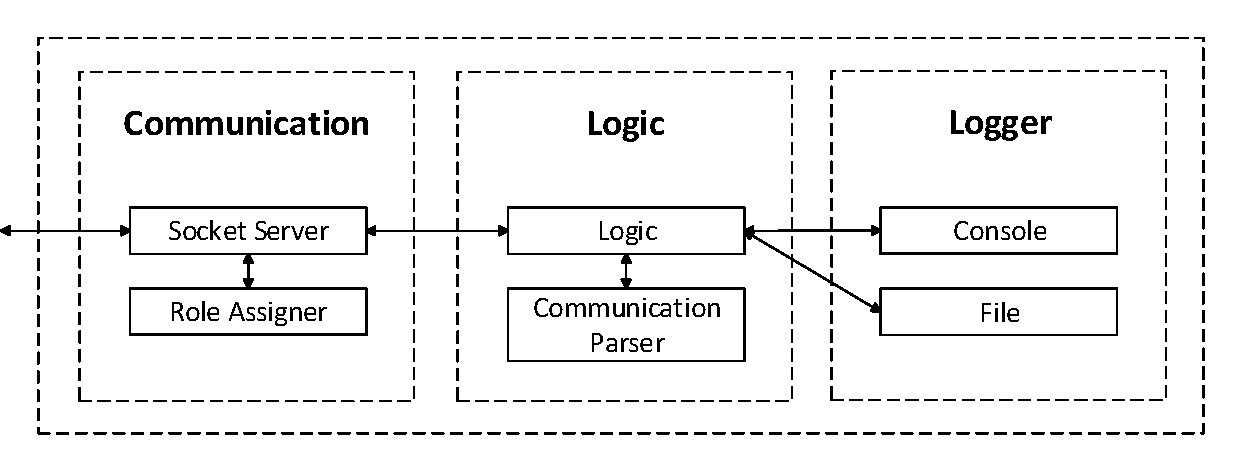
\includegraphics[width=\textwidth]{vector/blokoveSchemaSecurityServer.pdf}
\caption{Blokové schéma objektového návrhu komunikačního serveru}
\label{image}
\end{center}
\end{figure}

\subsection{Communication}
Blok „Communication“ obsahuje vlákno „Socket Server“, které poslouchá na portu 6666 a navazuje komunikaci přes technologii Socket. Server udržuje všechna spojení aktivní a stárá se o produkci všech zpáv až ke všem cílům. Pokud je některé spojení přerušeno, zajistí informování všech ostatních uživatelů a uvolní zdroje. 

„Role Assigner“ se stará o oddělení neidentifikovaných klientů od těch indetifikovaných. Identifikovaný klient se vyznačuje tím, že provedl autorizaci jako řídící jednotka, nebo mobilní aplikace. Dále se vyznačuje tím, že je mu umožněno komunikovat s ostatními protějšky, tedy řídící jednotka může kontaktovat všechny mobilní aplikace, a všechny mobilní aplikace mohou kontaktovat všechny řídící jednotky. Dokud není klient identifikovaný, není mu umožněno komunikovat s nikým jiným, než s komunikačním serverem.

\subsection{Logic}
Blok „Logic“ je hlavní vlákno, které řídí tok komunikace indetifikovanch klientů. Protékající data zpracovává a uchovává k zobrazení ve webové aplikac. Dále se stará o tisk komunikace na zvolených výstupech z bloku „Logger“.

\subsection{Logger}
Blok „Logger“ slouží k výpisu či logování probíhající komunikace a dalších informací. Aktuálně je možné výpis provádět do konzole, která je ideální pro ladění uživatelem, případně je možný výpis do souboru, kde slouží pro zpětné dohledávání chyb.

\section{Zprovoznění}
Pro správnou funkcionalitu komunikačního serveru, je nutné server provozovat na veřejné IP adrese, s přesměrováním portu 6666 na lokální adresu serveru v interní síti.

\section{Konzolový výstup}
Pro lepší vývoj a testování jsem vytvořil konzolový náhled na komunikaci serveru, kde jsou časově a barevně odlišeny různé operace.

\begin{figure}[H]
\begin{center}
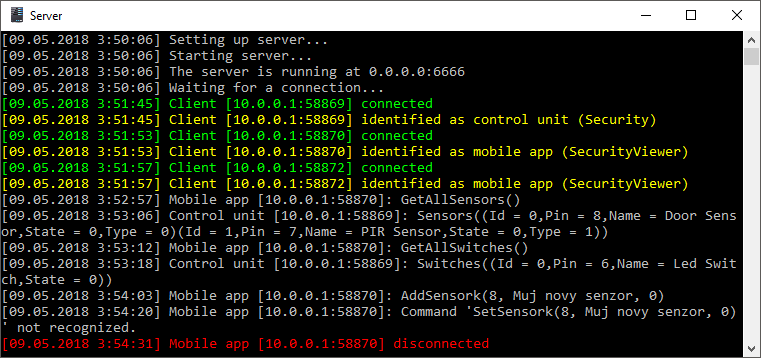
\includegraphics[width=\textwidth]{images/serverView.png}
\caption{Konzolové okno komunikačního server}
\label{image}
\end{center}
\end{figure}

\paragraph{Významy barev v serverovém logu:}
\begin{itemize}
\item Zelená - Zařízení připojeno
\item Žlutá - Zařízení identifikováno (řídící jednotka, nebo mobilní aplikace)
\item Červená - Zařízení odpojeno
\item Šedivá - Běžná komunikace
\end{itemize}

\section{Testovací klient}
Testovací klient vznik za účelem testování serverové části, bez nutnosti komunikace reálných zařízení nad reálnými daty. Klient umožňuje výběr z několika režimů, kde každý umožňuje simulovat něco jiného. Po výběru jednoho z režimů, se testovací klient připojí na komukační server pod zvoleným nastavením. Poté lze například zasílat testovací retěžce se seznamem komponent, odpovídat na API dotazy a podobné.

\paragraph{Seznam všech režimů testovacího klienta:}
\begin{itemize}
\item Simulace mobilní aplikace
\item Simulace mobilní aplikace (READ ONLY)
\item Simulace mobilní aplikace (WRITE ONLY)
\item Simulace řídící jednotky
\item Simulace řídící jednotky (READ ONLY)
\item Simulace řídící jednotky (WRITE ONLY)
\end{itemize}

\begin{figure}[H]
\begin{center}
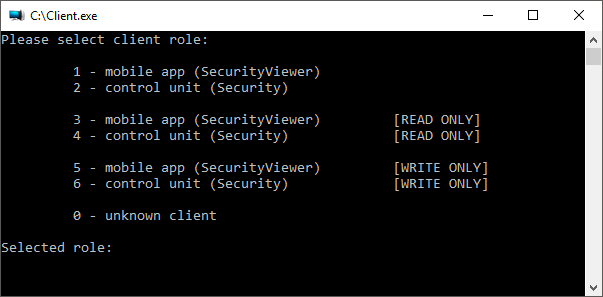
\includegraphics[width=\textwidth]{images/testingClient.png}
\caption{Konzolové okno testovacího klienta}
\label{image}
\end{center}
\end{figure}


% Závěr

\chapter{Závěr}
V rešeršní části jsem definoval zabezpečovací systém a inteligentní dům, ze kterých se sestává inteligentní domovní systém. Nakonec jsem definoval požadované vlastnosti jednotlivých součástí inteligentího domovního systému, kterými jsou domovní systém, desktopová aplikace, mobilní aplikace, webová aplikace a komunikační server. 

Na základě častých konzultací s vedoucím práce, jsem navrhl koncept cílového produktu, doporučil realizační postupy, vybral hardware, nebo uvedl více možností jeho výběru, kterými může být dosaženo výsledného zařízení. Následně jsem zvolil komunikační prostředky a architekturu jednotlivých komponentů.

V první fázi jsem na základě konceptu jsem zvolil nejvhodnější komponenty pro vývoj prototypu, které jsem následně zakoupil. Při práci na prototypu jsem odhalil, že jednen z původních cílů, využít tlačítkový mobilní telefon pro přístup do sítě GPRS, je nerealizovatelný, zvolil jsem tedy alternativní postup. Dále jsem vyvinul firmware řídící jednotky, který jsem úspěšně otestoval na prototypu. Po dopsání vlastního kódu jsem podrobně popsal všechny funkce programu.

V druhé fázi jsem vyvinul desktopovou aplikaci pro systém Windows, kterou jsem plně otestoval pro více verzí systému Windows 10, popsal všechny funkce programu a zajistil kompatibilitu pro starší verze systému Windows.

Třetí fáze zahrnovala tvrobu mobilní aplikace, u které jsem zjistil, že přímá komunikace aplikace a řídící jednotky je nerealizovatelná, proto jsem nejdříve vytvořil komunikační server pro systém Windows, který zprostředkovával požadované spoojení v síti internet. Následně jsem dokončil mobilní aplikaci pro systém Android. Aplikaci jsem plně otestoval, popsal všechny funkce a zajistil kompatibilitu u starších systémů.

Poslední fáze byla tvorba webového prostředí pro monitoring domácího systému. Webovou aplikaci, čerpající data z komunikačního serveru jsem otestoval a řádně popsal všechny její funkce.

Funkční prototyp, včetně všech příslušných aplikací jsem otestoval v běžném provozu.

Zadání se mi podařilo splnit ve všech bodech. Do budoucna bych rád předělal komunikační server ze systému Windows na běžnější formu serveru, kterou bude možné spustit na některé z hostingových služeb. Rád bych také vytvořil mobilní aplikaci pro systém iOS.

% Literatura

\addcontentsline{toc}{chapter}{Literatura}

\begin{thebibliography}{10}
\bibitem{Arduino intro}Arduino introduction. Arduino [online]. [cit. 2017-05-23]. Dostupné z: \url{https://www.arduino.cc/en/Guide/Introduction}
\bibitem{Arduino lib}Arduino libraries. Arduino [online]. [cit. 2016-05-08]. Dostupné z: \url{https://www.arduino.cc/en/Reference/Libraries}
\bibitem{ArduinoProducts}Arduino Products [online]. [cit. 2018-05-08]. Dostupné z: \url{https://www.arduino.cc/en/Main/Products}
\bibitem{Arduino lang}Arduino programming language. Arduino [online]. [cit. 2016-05-08]. Dostupné z: \url{https://www.arduino.cc/en/Reference/HomePage}
\bibitem{Arduino schematic}Arduino Schematic [online]. 1 s. [cit. 2016-05-07]. Dostupné z: \url{https://www.arduino.cc/en/uploads/Main/Arduino\_Uno\_Rev3-schematic.pdf}
\bibitem{Arduino soft} Arduino software. Arduino [online]. [cit. 2016-05-08]. Dostupné z: \url{https://www.arduino.cc/en/Main/Software}
\bibitem{Arduino source}Arduino source code. GitHub [online]. [cit. 2016-05-08]. Dostupné z: \url{https://github.com/arduino/Arduino/tree/1.6.8}
\bibitem{Atmega datasheet}ATmega48A/PA/88A/PA/168A/PA/328/P Datasheet [online]. 2015, 660 s. [cit. 2016-05-07]. Dostupné z: \url{http://www.atmel.com/images/Atmel-8271-8-bit-AVR-Microcontroller-ATmega48A-48PA-88A-88PA-168A-168PA-328-328P\_ datasheet\_Complete.pdf}
\bibitem{BaudRates}BaudRates for communicating with the computer [online]. [cit. 2018-05-08]. Dostupné z: \url{https://www.arduino.cc/en/serial/begin}
\bibitem{CompareBoardSpecs}Compare board specs [online]. [cit. 2018-05-08]. Dostupné z: \url{https://www.arduino.cc/en/Products/Compare}
\bibitem{DesktopMarketShare}Desktop Operating System Market Share Europe [online]. [cit. 2018-05-07]. Dostupné z: \url{http://gs.statcounter.com/os-market-share/desktop/europe/#monthly-201704-201804-bar}
\bibitem{Electronic security signalisation}Elektronická zabezpečovací signalizace. Wikipedia [online]. [cit. 2017-05-23]. Dostupné z: \url{https://cs.wikipedia.org/wiki/Elektronick\%C3\%A1\_zabezpe\%C4\%8Dovac\%C3\%AD_signalizace}
\bibitem{Electronic security system}Elektronické zabezpečovací systémy [online]. , 1 [cit. 2017-05-23]. Dostupné z: \url{http://www.ezasys.cz/elektronicke-zabezpecovaci-systemy/}
\bibitem{HTML1.1}FIELDING, R., UC IRVINE, J. GETTYS, et al. Hypertext Transfer Protocol -- HTTP/1.1 [online]. 1999, , 176 [cit. 2017-05-27]. Dostupné z: \url{http://www.ietf.org/rfc/rfc2616.txt}
\bibitem{TULVisual}Manuál jednotného vizuálního stylu Technické univerzity v Liberci [online]. , 27 [cit. 2017-05-27]. Dostupné z: \url{http://www.ft.tul.cz/document/126}
\bibitem{.NetFramework4.5.2}Microsoft .NET Framework 4.5.2. Microsoft.com [online]. [cit. 2018-02-21]. Dostupné z: \url{https://www.microsoft.com/en-us/download/details.aspx?id=42642}
\bibitem{MobileMarketShare}Mobile Operating System Market Share Europe [online]. [cit. 2018-05-07]. Dostupné z: \url{http://gs.statcounter.com/os-market-share/mobile/europe/#monthly-201704-201804-bar}
\bibitem{Bachelor thesis}MORAVEC, Tomáš. Koncept nízkonákladového sledovacího zařízení pro osobní automobily: The concept of a low cost tracking device for personal cars. Liberec: Technická univerzita v Liberci, 2016.
\bibitem{LaTeX}SATRAPA, Pavel. LaTeX pro pragmatiky [online]. 2011, 87 s. [cit. 2016-05-07]. Dostupné z: \url{http://www.nti.tul.cz/~satrapa/docs/latex/latex-pro-pragmatiky.pdf}
\bibitem{LaTeX}SATRAPA, Pavel. Stručný přehled příkazů LaTeXu [online]. 2011, 2 s. [cit. 2016-05-07]. Dostupné z: \url{http://www.nti.tul.cz/~satrapa/docs/latex/latex-prehled.pdf}
\bibitem{Security alarm}Security alarm. Wikipedia [online]. [cit. 2017-05-23]. Dostupné z: \url{https://en.wikipedia.org/wiki/Security_alarm}
\bibitem{SIMCOM SW}SIM908 AT Command Manual [online]. Jinzhong, 2011, 249 s. [cit. 2016-05-07]. Dostupné z: \url{http://www.dfrobot.com/image/data/TEL0051/3.0/SIM908\_AT\%20Command\%20Manua\_V1.01.pdf}
\bibitem{SIMCOM HW}SIM908 Hardware Design [online]. 2. Jinzhong, 2012, 53 s. [cit. 2016-05-07]. Dostupné z: \url{http://www.niplesoft.net/blog/wp-content/uploads/2016/02/SIM908-Hardware-Design-V2.00-1.pdf}
\bibitem{Visual Micro}Visual Micro [online]. [cit. 2017-05-23]. Dostupné z: \url{http://www.visualmicro.com/}
\bibitem{Pruvodce arduinem}VODA, Zbyšek. Průvodce světem Arduina [online]. Vydání první. Bučovice: Martin Stříž, 2015 [cit. 2016-05-07]. ISBN 978-80-87106-90-7.
\bibitem{WhatsNew.NetFramework4.5.2}What's new in the .NET Framework 4.5.2. Microsoft.com [online]. [cit. 2018-02-21]. Dostupné z: \url{https://docs.microsoft.com/en-us/dotnet/framework/whats-new/index#v452}
\bibitem{Wiring}Wiring [online]. [cit. 2016-05-08]. Dostupné z: \url{http://wiring.org.co/}
\end{thebibliography}

% Příloha

\appendix

\chapter{Obsah přiloženého CD}
Struktura a obsah adresářů je následující:

\paragraph{/Dokumentace}\mbox{}\\\mbox{}\\
Text bakalářské práce ve formátu pdf.

\paragraph{/Hardware}\mbox{}\\\mbox{}\\
Podklady k hardwaru.

\paragraph{/Hardware/Dokumentace (Datasheets)}\mbox{}\\\mbox{}\\
Hardwarová dokumentace od výrobců použitých součástek.

\paragraph{/Hardware/Fotografie}\mbox{}\\\mbox{}\\
Fotografie součástek, zapojení, informačních šťítků.

\paragraph{/Software}\mbox{}\\\mbox{}\\
Zdrojové kódy jednotlivých aplikací.

\paragraph{/Software/SecurityControl (Desktopová aplikace)}\mbox{}\\\mbox{}\\
Desktopová aplikace pro operační systém Windows.

\paragraph{/Software/SecurityDashboard (Webová aplikace)}\mbox{}\\\mbox{}\\
Webová aplikace pro online statistiky.

\paragraph{/Software/SecurityFirmware (Řídící jednotka)}\mbox{}\\\mbox{}\\
Firmware pro řídící jednotku Arduino.

\paragraph{/Software/SecurityServer (Komunikační server)}\mbox{}\\\mbox{}\\
Komunikační server a testovací klientská aplikace pro operační systém Windows.

\paragraph{/Software/SecurityViewer (Mobilní aplikace)}\mbox{}\\\mbox{}\\
Mobilní aplikace pro operační systém Android.

\end{document}